\documentclass[answers]{exam}
\usepackage{../MT2023}
\usepackage{graphicx}
\graphicspath{ {./images} }

\title{Geometry -- Sheet 4\\Isometries, Change of coordinates}
\author{YOUR NAME HERE :)}
\date{Michaelmas Term 2023}


\begin{document}
\maketitle
\begin{questions}

\question%1
\begin{parts}
\part%1a
Let \[
	A=\begin{pmatrix}
		1 & a & b \\
		c & d & -1 \\
		e & \frac{1}{2} & f
	\end{pmatrix}.
\] Are there constants $a, b, c, d, e, f$ such that $A$ is orthogonal?

\part%1b
If an orthogonal matrix represents a reflection, show that it is symmetric. Is the converse true?

\part%1c
Let $A$ be an $n \times n$ matrix for which there exists an orthogonal matrix $P$ such that $P^{T} A P$ is diagonal. Show that $A$ is symmetric.
\end{parts}



\question%2
\begin{parts}
\part%2a
Let $T: \mathbb{R}^{2} \to \mathbb{R}^{3}$ be the map given by \[
	T(\mathbf x)=A\mathbf x+\mathbf b\quad\text{where}\quad A=\begin{pmatrix}
		1 / 3 & 0 \\
		2 / 3 & 1 / \sqrt{2} \\
		2 / 3 & -1 / \sqrt{2}
	\end{pmatrix}\quad
	\text{and}\quad
	\mathbf b=\begin{pmatrix}
		1 \\
		1 \\
		1
	\end{pmatrix}.
\] Show that $A^{T} A=I_{2}$ and deduce that $T$ is an isometry. What is the image of $T$?

\part%2b
Show that there is no isometry from $\mathbb{R}^{3}$ to $\mathbb{R}^{2}$.
\end{parts}



\question%3
Let $\mathbf{e}_{1}, \mathbf{e}_{2}, \mathbf{e}_{3}$ be an orthonormal basis in $\mathbb{R}^{3}$ which is right-handed (so that $\mathbf{e}_{1} \wedge \mathbf{e}_{2}=\mathbf{e}_{3}$, $\mathbf{e}_{2} \wedge \mathbf{e}_{3}=\mathbf{e}_{1}$, $\mathbf{e}_{3} \wedge \mathbf{e}_{1}=\mathbf{e}_{2}$). Say that \[
	X\mathbf e_1+Y\mathbf e_2+Z\mathbf e_3=x\mathbf i+y\mathbf j+z\mathbf k\qquad
	\text{and}\qquad
	\tilde X\mathbf e_1+\tilde Y\mathbf e_2+\tilde Z\mathbf e_3=\tilde x\mathbf i+\tilde y\mathbf j+\tilde z\mathbf k.
\] Show that \[
	X \tilde{X}+Y \tilde{Y}+Z \tilde{Z}=x \tilde{x}+y \tilde{y}+z \tilde{z}
\] and \[
	(Y \tilde{Z}-Z \tilde{Y}) \mathbf{e}_{1}+(Z \tilde{X}-X \tilde{Z}) \mathbf{e}_{2}+(X \tilde{Y}-Y \tilde{X}) \mathbf{e}_{3}=(y \tilde{z}-z \tilde{y}) \mathbf{i}+(z \tilde{x}-x \tilde{z}) \mathbf{j}+(x \tilde{y}-y \tilde{x}) \mathbf{k}
\] What is the significance of these identities?



\question%4
Let $\mathbf{u}, \mathbf{v}$, and $\mathbf{w}$ be vectors in $\mathbb{R}^{3}$.
\begin{parts}
\part%4a
What does it mean to say that $\{\mathbf{u}, \mathbf{v}, \mathbf{w}\}$ forms a basis for $\mathbb{R}^{3}$?

\part%4b
Suppose a vector $\mathbf{x} \in \mathbb{R}^{3}$ has coordinates $(x_{1}, x_{2}, x_{3})$ in the basis $\{\mathbf{u}, \mathbf{v}, \mathbf{w}\}$. Give a formula for the length of $\mathbf{x}$ in terms of its coordinates and properties of $\mathbf{u}, \mathbf{v}, \mathbf{w}$. What properties of $\mathbf{u}, \mathbf{v}, \mathbf{w}$ are thus required in order for the usual length formula to hold? Hence or otherwise, determine the equation of the unit sphere in the coordinate system defined by the basis $\{\mathbf{u}, \mathbf{v}, \mathbf{w}\}$.

\part%4c
Suppose $\{\mathbf{u}, \mathbf{v}, \mathbf{w}\}$ and $\{\mathbf{U}, \mathbf{V}, \mathbf{W}\}$ are both orthonormal bases in $\mathbb{R}^{3}$, with coordinates given by $\mathbf{x}=(x_{1}, x_{2}, x_{3})$ and $\mathbf{X}=(X_{1}, X_{2}, X_{3})$, respectively. By considering the transformation of coordinates in converting from one basis to the other, show that the equation of the unit sphere is invariant.
\end{parts}



\question%5
Let $\mathbf{n}$ be a unit vector in $\mathbb{R}^{3}$. The stretch $S_{k}$ with invariant plane $\mathbf{r} \cdot \mathbf{n}=c$ and stretch factor $k$ is defined by \[
	S_{k}(\mathbf{v})=\mathbf{v}+(k-1)(\mathbf{v} \cdot \mathbf{n}-c) \mathbf{n}
\]
\begin{parts}
\part%5a
Describe the maps $S_{1}, S_{0}$ and $S_{-1}$.

\part%5b
Determine the matrix for $S_{k}$ when the invariant plane is $x+y+z=0$.

\part%5c
Find an orthonormal basis $\mathbf{e}_{1}, \mathbf{e}_{2}, \mathbf{e}_{3}$ of $\mathbb{R}^{3}$ such that $\mathbf{e}_{1}, \mathbf{e}_{2}$ are parallel to the plane in (b). Describe the map $S_{k}$ in terms of the co-ordinates associated with $\mathbf{e}_{1}, \mathbf{e}_{2}, \mathbf{e}_{3}$.
\end{parts}



\question%6
(Optional) Consider the system of differential equations \[
	\begin{pmatrix}
		x_{1}''(t) \\
		x_{2}''(t) \\
		x_{3}''(t)
	\end{pmatrix}=\frac{g}{m l}\begin{pmatrix}
		-1 & 1 & 0 \\
		1 & -3 & 2 \\
		0 & 2 & -5
	\end{pmatrix}\begin{pmatrix}
		x_{1}(t) \\
		x_{2}(t) \\
		x_{3}(t)
	\end{pmatrix},
\] which we could abbreviate $\mathbf{x}''(t)=\frac{g}{m l} A \mathbf{x}(t)$. These equations provide a simple model of the dynamics of a 'triple pendulum', a system of 3 equal masses $m$ hanging under the force of gravity $g$ and connected by strings of length $l$ (see the figure below). The variables $x_{i}(t)$ denote the horizontal displacement.
\begin{center}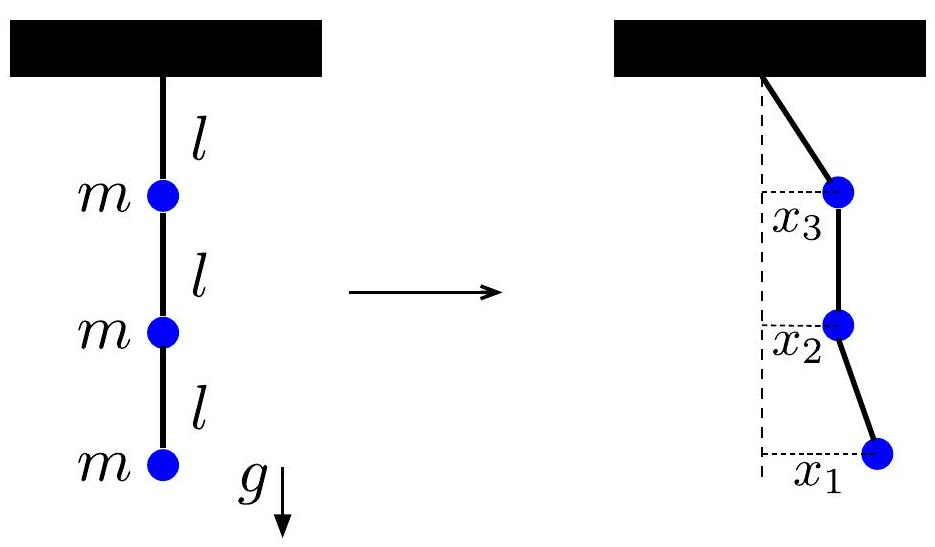
\includegraphics[scale=0.25]{sheet 4 diagram}\end{center}
Noting that $A$ is symmetric, Spectral Theory gives us that $A$ can be expressed as $A=P D P^{T}$ for an orthogonal matrix $P$ and diagonal matrix \[
	D=\begin{pmatrix}
		-\lambda_{1} & 0 & 0 \\
		0 & -\lambda_{2} & 0 \\
		0 & 0 & -\lambda_{3}
	\end{pmatrix}
\] and in this case the $\lambda_{i}>0$. Use this fact to determine the general solution for $\mathbf{x}(t)$. [You need not explicitly compute $P$ or the $\lambda_{i}$.]

\end{questions}

\end{document}
